\subsection{The Transfer Testbed}
The transfer testbed was upgraded in March 2015. Until then, it operated with gridFTP transfers between all sites, providing a low-level test of connectivity and functionality for the almost two years that it ran. Since March 2015 the testbed uses FTS3 to initiate the transfers, moving up the middleware stack. Since FTS3 is used for the vast majority of experiment transfers in WLCG this provides an important full-stack test.

At the present time, the testbed consists of 7 storage elements at sites distributed around Europe. One is IPv6-only, the rest are all dual-stack. All the SEs are running dCache. Most are stable installations, but one (DESY) is rebuilt every morning with the latest patches from dCache, providing a valuable regression-test for both the dCache and IPv6 teams.

As before, each site serves as both a source and a destination, with each source sending a 1~GB file to each destination. The file-size is validated at the destination using {\bf gfal-ls}, then the destination is cleaned with {\bf gfal-rm} and the transfer duration is recorded. Then the cycle is repeated after a short delay, to avoid abusing the hardware/network with too much traffic. Physical file names are specified using the SRM protocol.

Two FTS3 servers are deployed for the testbed, one at Imperial College and one at KIT, though currently only the one at KIT is used.

Figure.~\ref{fig:fts3-mesh} shows the transfers in the FTS3 testbed so far. Most sites transfer efficiently in both directions, but the effect of the firewall at KIT on inbound traffic can be clearly seen.

\begin{figure}[h]
 \centering
   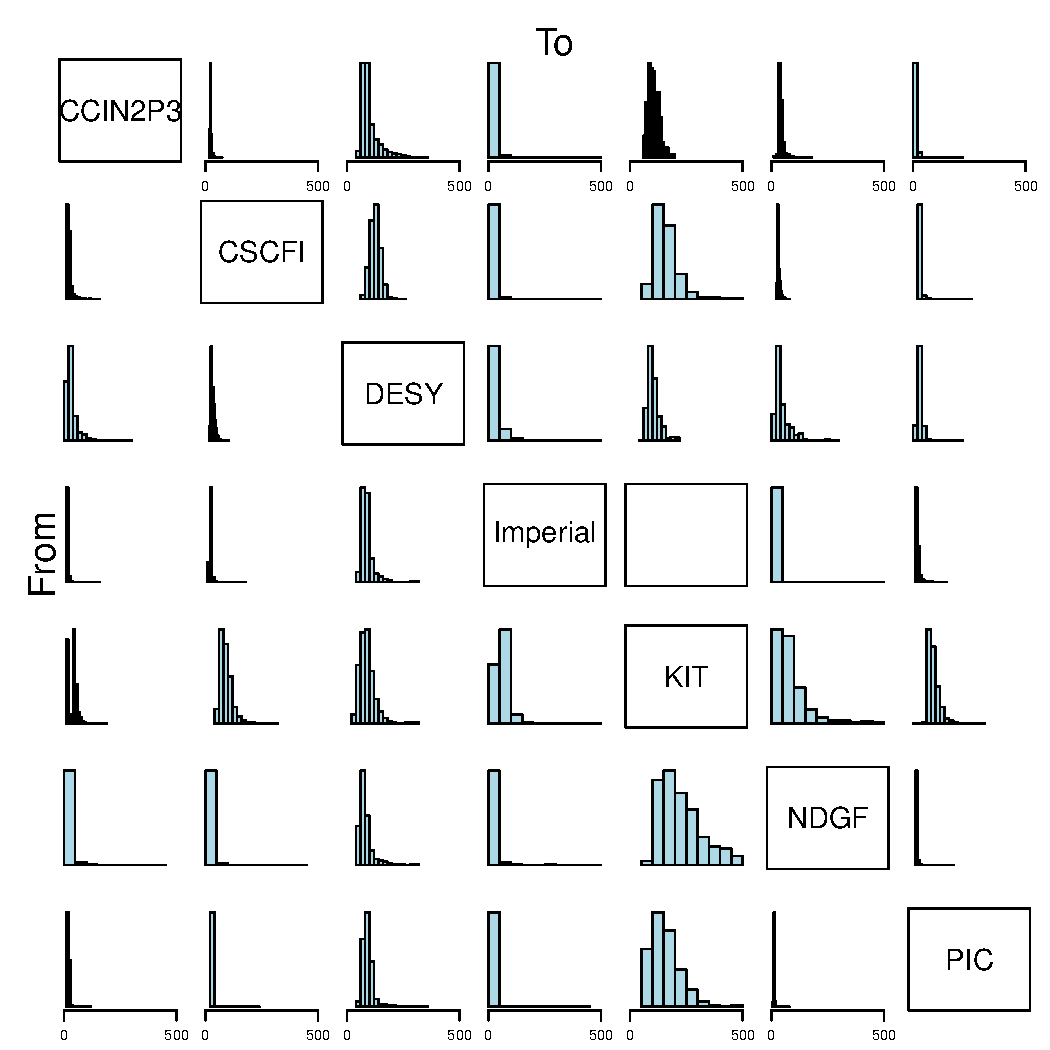
\includegraphics[width=0.8\textwidth]{fts3-mesh.pdf}
       \caption{The FTS3 transfer testbed. Rows show transfers from the named site, columns show transfers to the destination. The horizontal axis for all plots is fixed at 500 seconds, i.e. transfers that proceed at less than 2 MB/sec will overflow.}
 \label{fig:fts3-mesh}
\end{figure}


\subsection{FTS3 server and dCache SE at KIT}
For managing file transfers between sites, an FTS3 instance is setup at KIT. Furthermore, a storage element based on dCache 2.10 on Scientic Linux is created. Both instances are rolled out on physical machines.

\subsubsection{FTS3}
FTS3 supports IPv6 in its baseline version. The service has to bind to IPv6 locally in the FTS3 conguration (IP=::) and to be enabled explicitely for gfal.2 ( IPV6=true). The host is available in the DNS as default dual-host, with IP4 and IPv6 announced in the A and AAAA records, and also with IPv4-only or IPv6-only names with an -ipv4 or -ipv6 appendix, respectively. Thus, all aliases have to included in the host certicate.

File transfers are successfully brokered by the FTS3 instance via IPv4 and IPv6 between the sites. Since most FTS3 instances in production use a separated database instance for performance and failsafe reasons, moving the database to a dedicated machine was tested as well. For the SQL db backends supported by FTS3, IPv6 support had been implemented in MySQL v5.5.3 and MariaDB v5.5.35, which are not available in the baseline SL6 repositories. MariaDB was installed on a dedicated host with version 5.5.42. After binding mysql locally to IPv6 as well ([mysqld] bind-address = ::), the database could be connected remotely with an IPv6-ready mysql client. For the FTS3 service to connect to the remote database via IPv6, the address has to be escaped explicitly, i.e., encapsulating the IP as [IP6]:PORT/fts3 and may depend on the version of the database library used by the FTS3 service.

\subsubsection{dCache based SE}
A dCache instance is setup on a dedicated host. The main hurdle for file transfer access was a reverse lookup by the instance when receiving a file request. After explicitely setting the dual-stack, IPv4-only, and IPv6-only host names in the dCache congfiguration (srm.net.local-hosts=hostname-ipv4,ipv6) and the general hosts file, the storage element is accessible via IPv4 and IPv6 as well.
